% Article type supporting font formatting
\documentclass[a4paper,11pt]{extarticle}

% Define .tex file encoding
\usepackage[utf8]{inputenc}

% Norwegian language support
%\usepackage[norsk]{babel}

% Sample text
\usepackage{lipsum}  

% Margin defining package
\usepackage{geometry}
\geometry{a4paper,margin=2cm}

% Better bibliography 
\usepackage[round]{natbib}

% For use of graphics in document
\usepackage{graphicx}

% Allows \begin{figure}[H]
\usepackage{float}

% For use of subfigures in document
\usepackage{subcaption}

% Allows easy writing of algorithms
\usepackage[ruled]{algorithm2e}

% Math related tools and functions
\usepackage{mathtools}

% Allows math in tex file 
\usepackage{amsmath}

% Allows math symbols in tex file
\usepackage{amssymb}

% Allows use of physics shortcut functions
%\usepackage{physics}

% For quotations
\usepackage{csquotes}

% Allows multi-line comments in tex file
\usepackage{verbatim}

% Verbatim env with LaTeX commands
\usepackage{alltt}

% Allows more control over tables
\usepackage{tabulary}

% Ads ul which allows line breaks while underlining text.
\usepackage{soul}

% Adds labeling list to the report
\usepackage{scrextend}
\addtokomafont{labelinglabel}{\ttfamily}

% Allows number referencing the last page, used in footer
\usepackage{lastpage}

% No indentation for the paragraphs, set distance between paragraphs
\usepackage{parskip}[skip=6pt]

% Adds "Appendix" before numbering for sections in appendix, use appendices env
\usepackage[title,toc,titletoc]{appendix}

% Change caption size and style
\usepackage[font=footnotesize,labelsep=period]{caption}

% Makes matrices look square-ish
\renewcommand*{\arraystretch}{1.5}

% Change date style
\usepackage[yyyymmdd]{datetime}
\renewcommand{\dateseparator}{-}

% Necessary for defining colours
\usepackage{xcolor}
\definecolor{linkgreen}{rgb}{0,.5,0}
\definecolor{linkblue}{rgb}{0,0.25,1}
\definecolor{linkred}{rgb}{.5,0,0}
\definecolor{blue}{rgb}{.13,.13,1}
\definecolor{green}{rgb}{0,.5,0}
\definecolor{red}{rgb}{.9,0,0}

% Hyperlinks in document
\usepackage{hyperref}
\hypersetup{
  colorlinks=true,     % True for colored links
  linktoc=all,         % True for table of contents links
  linkcolor=linkblue,  % Colour for links
  urlcolor=linkgreen,  % Colour for URLs
  citecolor=linkred    % Colour for citations
}

% Listing package for code examples
\usepackage{listings}         
\lstset{
  language=C++,                       % Set language to C++
  showspaces=false,                   % Don't show space chars
  showtabs=false,                     % Don't show tab chars
  breaklines=true,                    % Break long lines of code
  showstringspaces=false,             % Don't show spaces in strings
  breakatwhitespace=true,             % Break at white space only
  commentstyle=\color{green},         % Set colour for comments
  keywordstyle=\color{blue},          % Set colours for keywords
  stringstyle=\color{red},            % Set colour for strings
  basicstyle=\footnotesize\ttfamily,  % Set basic style
  tabsize=4                           % Set tabsize
}

% Allows editing of section headers
\usepackage{titlesec}
\titleformat*{\section}{\normalsize\bfseries}
\titleformat*{\subsection}{\normalsize\itshape\bfseries}
\titleformat*{\subsubsection}{\normalsize\bfseries}

% Change look and feel of abstract
\usepackage{abstract}
\setlength{\absleftindent}{0mm}
\setlength{\absrightindent}{0mm}
\renewcommand*\abstractname{\flushleft\normalsize\textbf{Abstract}\hfill}

% Allows editing of header and footer data
\usepackage{fancyhdr}
\fancypagestyle{plain}{
  \fancyhf{}
  \renewcommand{\headrulewidth}{0pt}
  \rfoot[R]{\footnotesize Page \thepage\ of \pageref*{LastPage}}
}
\pagestyle{fancy}
\fancyhf{}
\chead{\footnotesize Kristoffer Berg Wilhelmsen, Project in Fluid Mechanics, UiT Narvik 2022}
\rfoot{\footnotesize Page \thepage\ of \pageref*{LastPage}}
\setlength{\headheight}{20pt}
\setlength{\footskip}{20pt}

% Referencing, last for compatibility reasons
\usepackage[noabbrev,nameinlink]{cleveref}

%%%%%%%%%%%%%%%%%%%%%%%%%%%%%%%%%%%%%%%
%%      Title, Author, and Date      %%
%%%%%%%%%%%%%%%%%%%%%%%%%%%%%%%%%%%%%%%
\title{Visualization of downdraft from AW101 SAR Queen helicopter}
\author{Kristoffer Berg Wilhelmsen}
\date{\parbox{\linewidth}{\centering
    \textit{\small UiT - The Arctic University of Norway, P.O. Box 385, N-8505 Narvik, Norway}\endgraf\bigskip
    \small Submitted \today
}}
\providecommand{\keywords}[1]{\flushleft\textit{\small{Keywords:}} #1}

%%%%%%%%%%%%%%%%%%%%%%%%%%%%%%%%%%%%%%%
%%           Start document          %%
%%%%%%%%%%%%%%%%%%%%%%%%%%%%%%%%%%%%%%%
\begin{document}

%%%%%%%%%%%%%%%%%%%%%%%%%%%%%%%%%%%%%%%
%%   Create the main title section   %%
%%%%%%%%%%%%%%%%%%%%%%%%%%%%%%%%%%%%%%%
\maketitle

%%%%%%%%%%%%%%%%%%%%%%%%%%%%%%%%%%%%%%%
%%      Abstract for the report      %%
%%%%%%%%%%%%%%%%%%%%%%%%%%%%%%%%%%%%%%%
\noindent\rule{\linewidth}{.5pt}
\begin{abstract}
  The SAR Queen is a rescue helicopter set to replace the Sea King. Despite being an upgrade, it has its flaws. The helicopter creates a significantly stronger downdraft than its predecessor's, which can pose a danger to human life. Using visualization techniques from the Applied Computer Science curriculum, the objective is to identify how the downdraft affects pedestrian areas and the patient entrance of the hospital tunnel at the University Hospital of Northern Norway in Tromsø. The results from the techniques applied show that the downdraft has a varying effect on the areas. The pedestrian areas are affected the most during the initial and the final stages of landing, while the patient entrance is affected the most at a point in between.

  \keywords{\small{Fluid Mechanics}; \small{SAR Queen}; \small{AW101}; \small{Sea King}; \small{FLOW-3D}; \small{Python}; \small{Godot}; \small{imageio}}
\end{abstract}
\rule{\linewidth}{.5pt}

%%%%%%%%%%%%%%%%%%%%%%%%%%%%%%%%%%%%%%
%%  The main content of the report  %%
%%%%%%%%%%%%%%%%%%%%%%%%%%%%%%%%%%%%%%

\section{Introduction}
The AW101, domestically known as the Search \& Rescue (SAR) Queen in Norway, is a helicopter specialized for use in rescue missions \citep{ProjectDescription}. It is a replacement for Norway's previous rescue helicopter, known as the Sea King. The SAR Queen, seen in Figure \ref{fig:SarQueen}, is designed to fly long distances, withstand the arctic climate, strong winds and rough seas.
% Designed to fly long distances, withstand the arctic climate, strong winds and rough seas, the SAR Queen is essentially "The Terminator" of rescue helicopters. The helicopter can be seen in Figure \ref{fig:SarQueen}.

\begin{figure}[H]
  \centering
  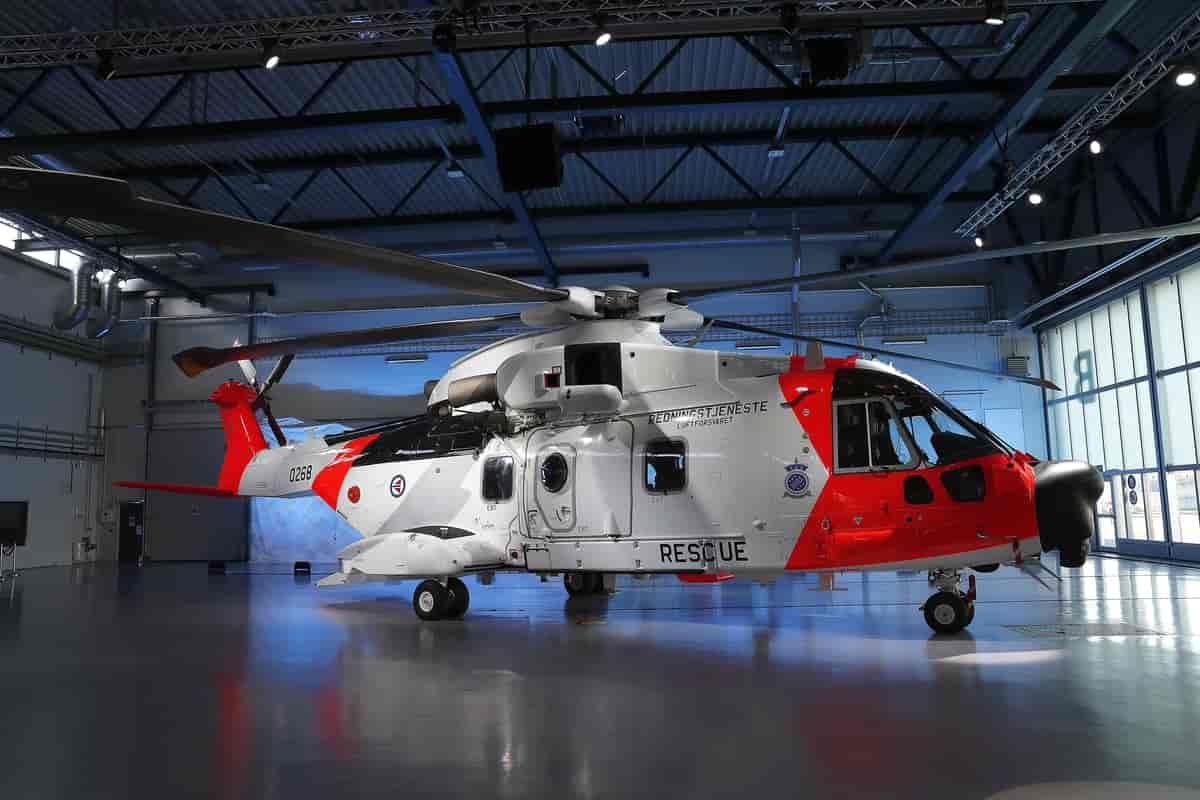
\includegraphics[width=0.8\textwidth]{gfx/sar_queen.jpg}
  \caption{The AW101 helicopter, also known as the SAR Queen \citep{AW101}.}
  \label{fig:SarQueen}
\end{figure}

% Despite the SAR Queen being a phenomenal helicopter for its intended area of use, it unfortunately also has its downsides. The downdraft created by the helicopter is much more significant than its predecessor's, and can be a potential danger for humans in proximity.
Unfortunately, the SAR Queen also has its downsides. The downdraft created by the helicopter is much more significant than its predecessor's, and can be a potential danger for persons in proximity. An article published by NRK \citep{NRK:SarQueen} mentions test landings from 2019 at St. Olav's University Hospital and Haukeland University Hospital, where the conditions were deemed unsafe for persons close by during landing, as a direct consequence of the helicopter's downdraft.

The objective of the work is to analyze the given flow problem, which takes place at the University Hospital of Northern Norway in Tromsø. Results from a numerical simulation using sensor data from a real landing was provided by professor Per-Arne Sundsbø, along with the 3D models used in the simulation. The results from the simulation and the models used are attached in Appendices \ref{app:simdata} and \ref{app:models}. By applying modern visualization techniques from the Applied Computer Science curriculum to create alternate visualizations, the analysis will look to determine how the helicopter's downdraft affects pedestrians in proximity and the hospital tunnel's patient entrance during landing.
%The objectives of the work are to perform post-processing on data obtained from a simulation.

\section{Material \& Methods}
Various pieces of software have been used in order to perform the analysis of the given problem. This section describes which software was used, to what extent, and how the results were obtained.

\subsection{Blender}\label{sec:Blender}
Blender \citep{blender} is a modelling application that can be used to create and animate 3D models. In order to use the supplied 3D models for animation purposes, their formats must be compatible with the software we intend on using. In this case we will use Godot to create animations, which does not currently support the models' \textit{stl} format. Godot's preferred format for 3D models is \textit{glTF} (.glb file extension). Converting the models can easily be done by importing them to Blender, and exporting them to the desired format.

\subsection{FLOW-3D}\label{sec:Flow3D}
FLOW-3D \citep{Flow3D} is an application used in computational fluid dynamics that has produced the raw data which forms the basis for the animations in the report. Due to the application being quite advanced, its use in this report outside providing data has been limited. It is also important to note that the application has not been a part of the curriculum, and licenses were not facilitated for use on personal computers. Thus, due to the short timeframe of this project, its limited use is reasonable. It has however also been used to create a similar animation to what we seek to obtain as a part of the work's main objective.

The raw data exported from FLOW-3D contains XYZ-coordinates corresponding to individual cells in the mesh pictured in Figure \ref{fig:Flow3DModel}, with associated values for volume fraction (float) and velocity magnitude (UVW-vector). Despite reducing the area that data is exported from drastically, each text file containing data for a single time step corresponded to $\sim$78 megabytes. The timeframe we want to animate is approximately 14.4 seconds long, with a step size of 0.4. This implies that there will be $\sim$36 different time steps, setting the cumulative file size to $\sim$2.8 gigabytes. In our case, a file of such a large size is not only undesirable to work with, but the format of its data must also be processed.

\begin{figure}[H]
  \centering
  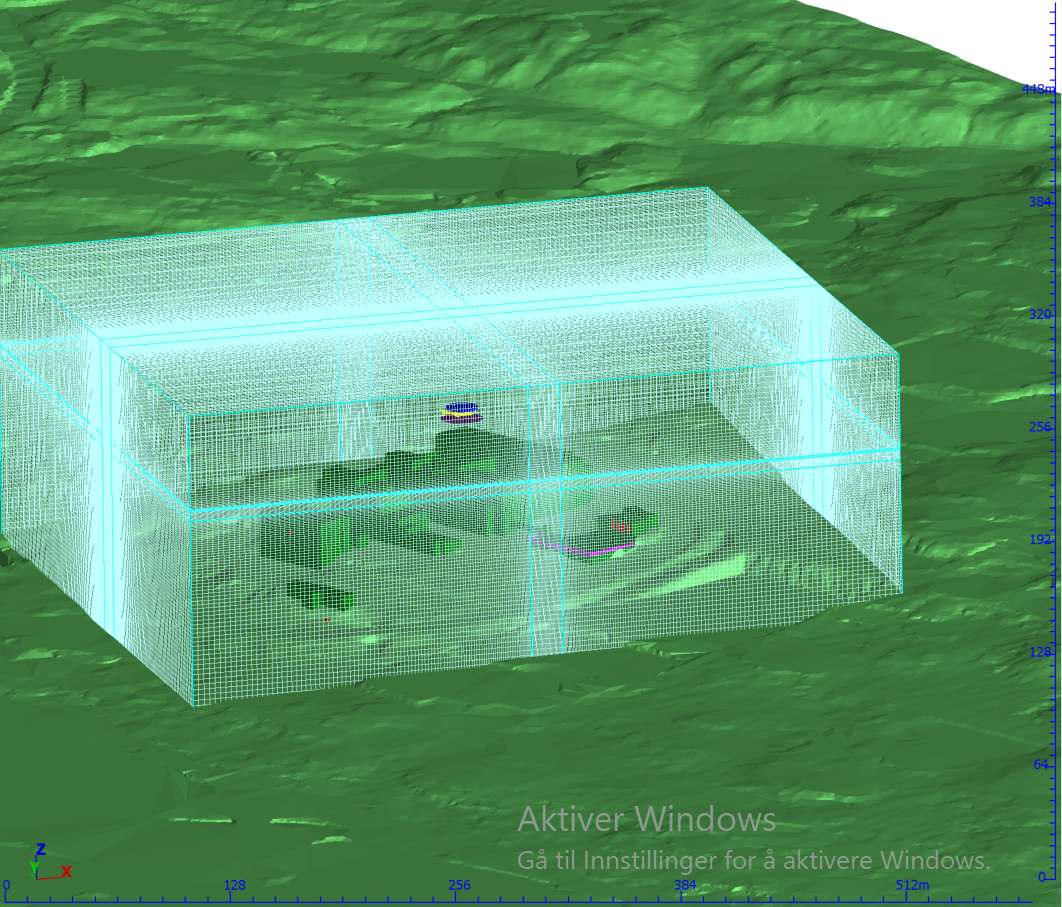
\includegraphics[width=0.8\textwidth]{gfx/flow3d_model.png}
  \caption{Model setup in FLOW-3D.}
  \label{fig:Flow3DModel}
\end{figure}

\subsection{Python}\label{sec:Python}
Python \citep{Python} is a programming language that is frequently used within data science, making it an excellent choice to further process the FLOW-3D data. As explained in Section \ref{sec:Flow3D}, the FLOW-3D output corresponds to individual cells in the mesh from Figure \ref{fig:Flow3DModel}. This includes cells that are not a part of the surface, which we are not interested in.

To filter out non-surface values, we can use the associated volume fraction. This is a float value from 0.0 to 1.0, which specifies how much of the cell is filled. If the volume fraction is 0.0, the cell is empty, hence is in the air. A volume fraction of 1.0 means that the cell is below the surface, as the entire cell is filled. To find values at the surface, we need to find XYZ-coordinates with an associated volume fraction that is in between.

Each cell's velocity magnitude is given in vector form, as mentioned in Section \ref{sec:Flow3D}. The color of a given point on the surface solely depends on the length of this vector ($\sqrt{u^2 + v^2 + w^2}$), which means that we can calculate it at this step to further reduce the size of the processed file.

After filtering out the non-surface values and calculating the length of the velocity magnitude vectors by using the script in Appendix \ref{script:process}, the file size for a single time step is reduced by $99\%$ ($\sim$78 megabytes $\rightarrow  \sim$ 600 kilobytes).

Using the processed data, we can create a texture to color the corresponding areas on the 3D models. A texture is simply an image with color values. To create the texture, we must determine its dimensions. First, we use the script in Appendix \ref{script:dimensions} to find the minimum and maximum value for the X- and Y-direction, as well as the minimum distance between values in the data set. By finding the difference between the minimum and maximum value in both directions and dividing it by the minimum distance, we find the texture dimensions. The minimum distance is a consequence of the mesh having more detail around the helipad. In this case the calculations are as follows:

\begin{itemize}
  \item X-min $= -60.43$, X-max $=53.56$, X-diff $\approx 114$
  \item Y-min $= -61.22$, Y-max $=66.37$, Y-diff $\approx 128$
  \item Minimum distance between values $= 0.62$
  \item X $= \frac{114}{0.62} \approx 184$, Y $= \frac{128}{0.62} \approx 206$
\end{itemize}

Note that X-diff, Y-diff, X and Y have been cast to integers due to the fact that image dimensions can not be floats. The script in Appendix \ref{script:texture} creates a NumPy \citep{numpy} matrix according to the calculated X and Y dimensions. Subsequently, the processed data containing XYZ-coordinates and velocity magnitude is read and placed in the NumPy matrix at indices relative to where the coordinates would be on the original FLOW-3D surface.

To calculate the texture dimensions, we used the smallest distance between values. This implies that there are greater distances in the data, resulting in gaps between indices in the texture. This is illustrated in Figure \ref{fig:PythonTextureGaps}, which has been generated using the Python library imageio \citep{imageio}.

\begin{figure}[H]
  \centering
  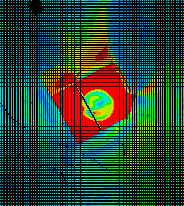
\includegraphics[width=0.8\textwidth]{gfx/uneven_texture.png}
  \caption{Texture with gaps in between indices.}
  \label{fig:PythonTextureGaps}
\end{figure}

A possible way of filling in the gaps is to copy nearby values. We can do this by sequentially iterating over each axis in the NumPy matrix, setting each empty value equal to the closest non-empty value. Figure \ref{fig:PythonTexture} illustrates a complete texture where empty indices have been filled.

\begin{figure}[H]
  \centering
  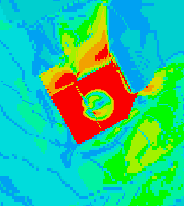
\includegraphics[width=0.8\textwidth]{gfx/texture.png}
  \caption{Example of a texture created in Python.}
  \label{fig:PythonTexture}
\end{figure}

\subsection{Godot}
Godot \citep{godot} is a game engine which primarily is used for game development. However, we can also use Godot to create animations. We set up the initial environment by importing the models converted in Section \ref{sec:Blender}. Additionally, we import the textures created in Section \ref{sec:Python}.

Tween \citep{godot:tween} and Timer \citep{godot:timer} are two types of objects in Godot. A Tween can be used to interpolate values (e.g. movement), and a Timer can be set to execute code when its timer expires. To simulate the movement of the helicopter, a Tween interpolates the values in between the helicopter's initial and final position from 0 to 14.4 seconds. The Timer triggers every 0.4 seconds (equivalent to a time step), and updates the texture to the corresponding time step.

A shader \citep{godot:shader} is a computer program that operates on the graphics card, performing tasks such as setting colors. To map the current texture to the buildings and the terrain, we can make use of shaders. The shader program operates in two steps. First, the vertex shader is executed, allowing the program to manipulate individual vertices. Here, we store the current position. Next, the fragment shader is executed, which colors individual pixels between vertices. In the fragment shader we check if the current position is within a set of bounds we define. Note that in this case, the data from FLOW-3D did not translate well to Godot. As such, the bounds for the texture have been determined by trial and error. Lastly, the pixels are colored by translating the current position to UV-values. These values range from 0.0 to 1.0 (floats), and correspond to a color on the texture.

The Godot project's repository can be found in Appendix \ref{src:godot}.

\subsection{OBS Studio}
OBS Studio \citep{obs} is a multipurpose application that can be used both for livestreaming and video recording. To capture the animations made throughout the project, OBS Studio has been used to record videos, which have then been uploaded to YouTube.

\section{Results \& Discussion}\label{sec:results}
% The Godot animation is the main result from the project work. The first time step from the animation can be seen in Figure, and the last time step can be seen in Figure.
% Figure shows a frame of the Godot animation from an alternate angle.
% FLOW-3D animations as seen in Figure and Figure are equivalent to Figure and Figure from Godot, and have been added for comparison purposes.
The main results from the project work are the Godot animations. Supplementary animations from FLOW-3D have been added for comparisons.

\begin{figure}[H]
  \centering
  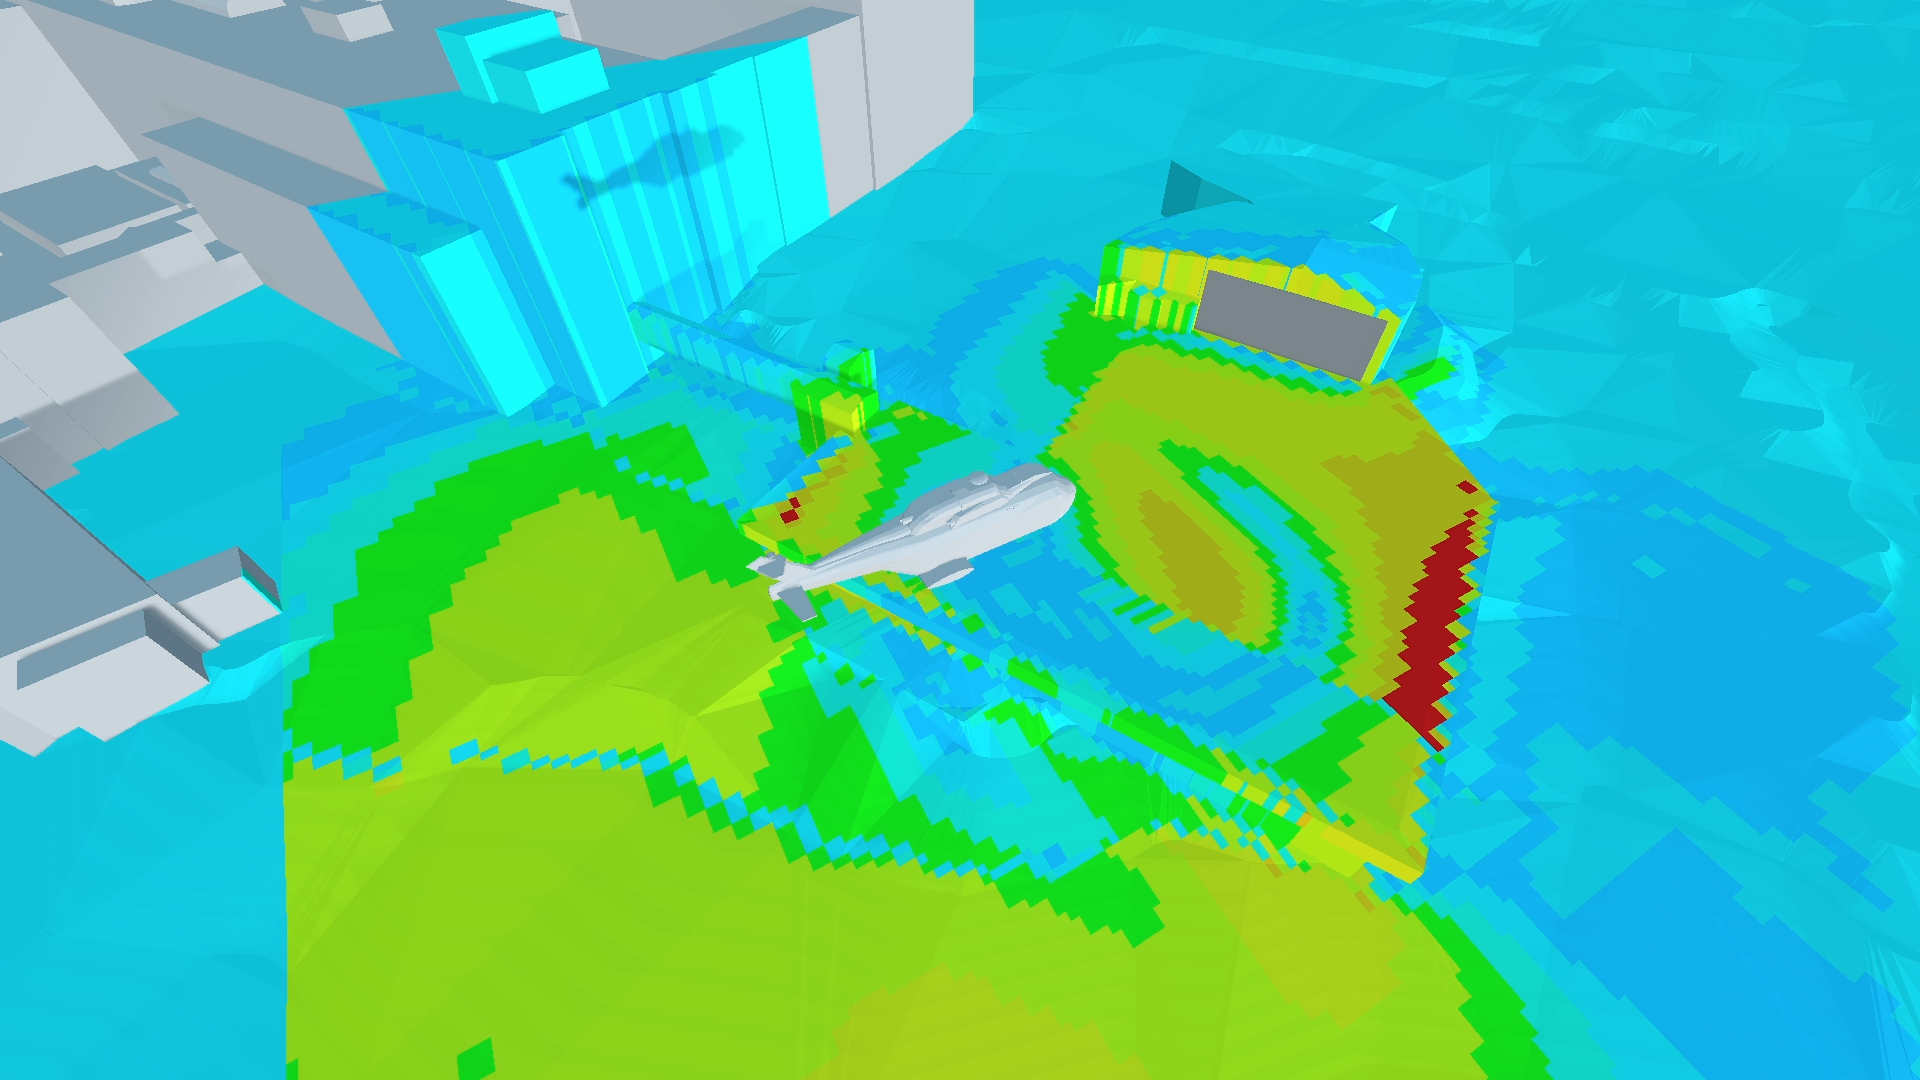
\includegraphics[width=0.8\textwidth]{gfx/anim_heli_first.png}
  \caption{Start of Godot animation with the camera attached to the helicopter.}
  \label{fig:AnimHeliFirst}
\end{figure}

\begin{figure}[H]
  \centering
  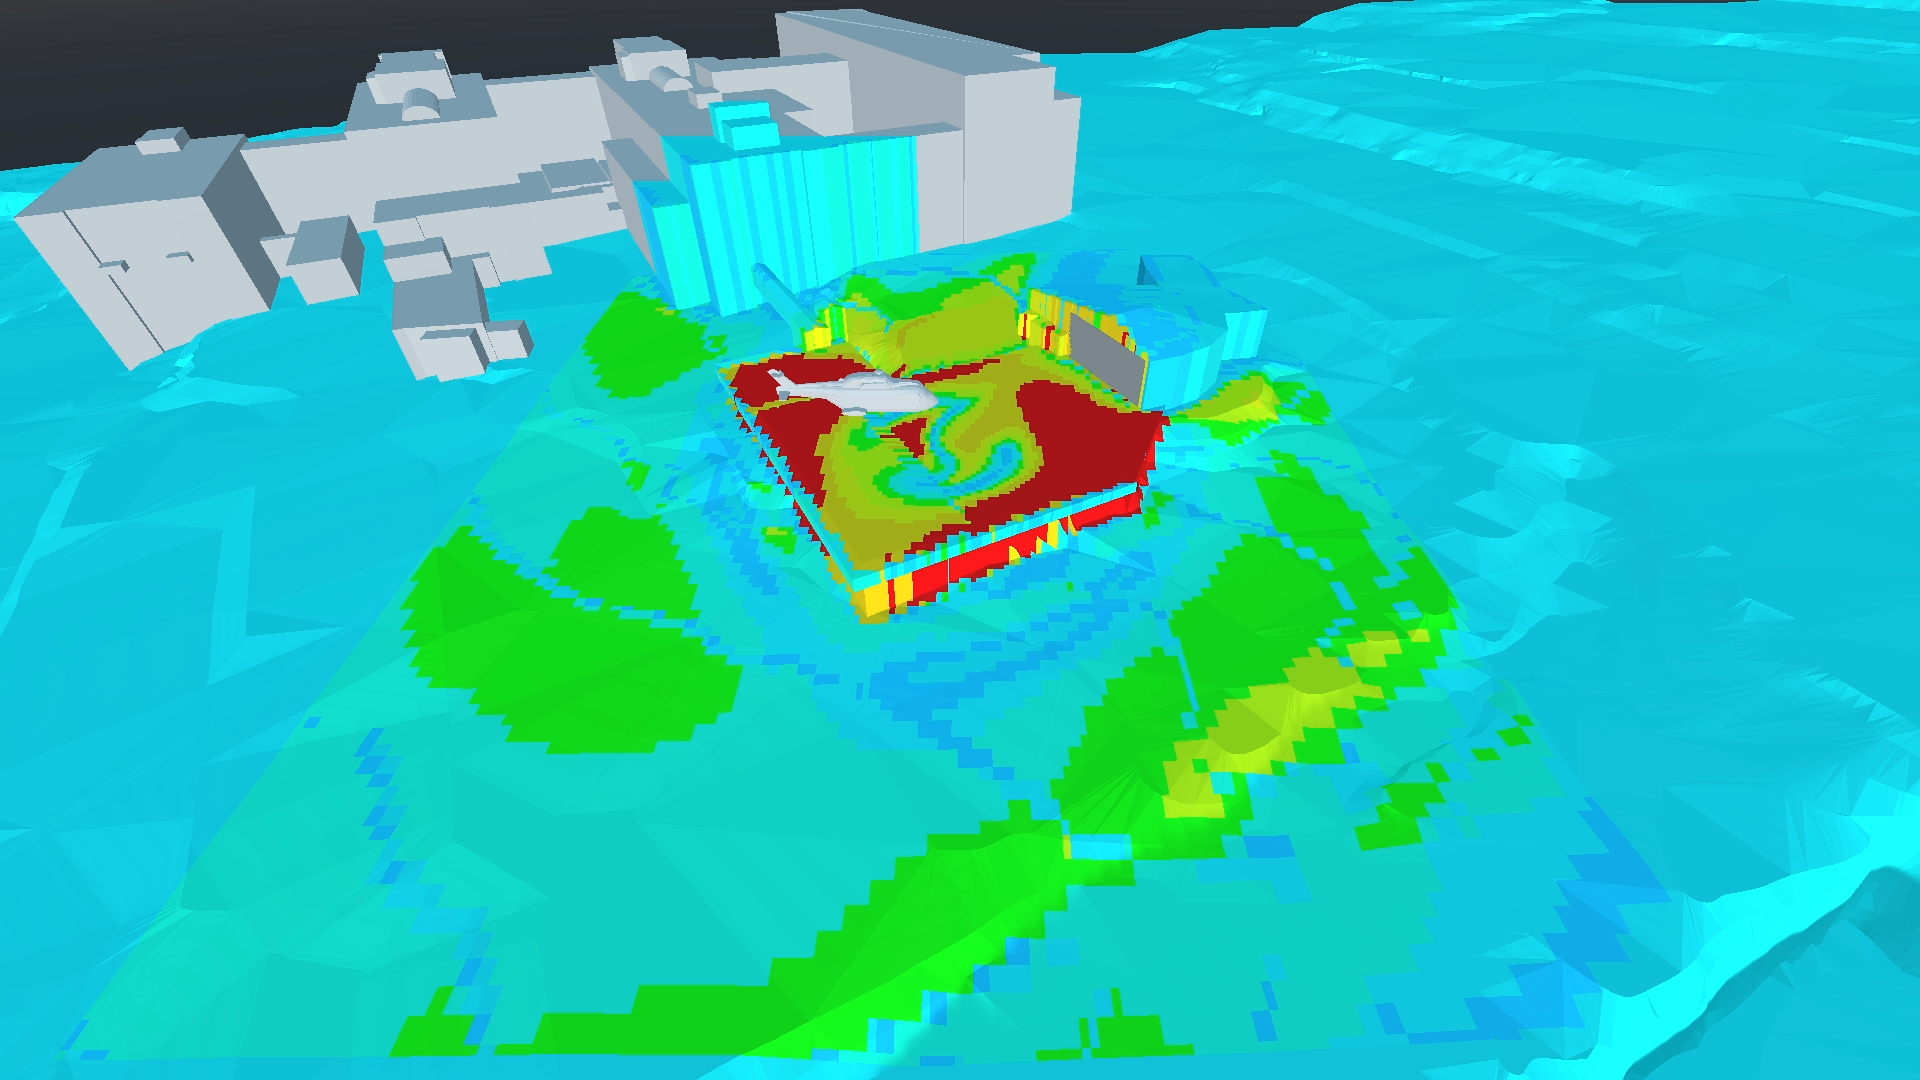
\includegraphics[width=0.8\textwidth]{gfx/anim_side_mid.png}
  \caption{Midpoint in Godot animation with stationary camera to the side.}
  \label{fig:AnimSideMid}
\end{figure}

\begin{figure}[H]
  \centering
  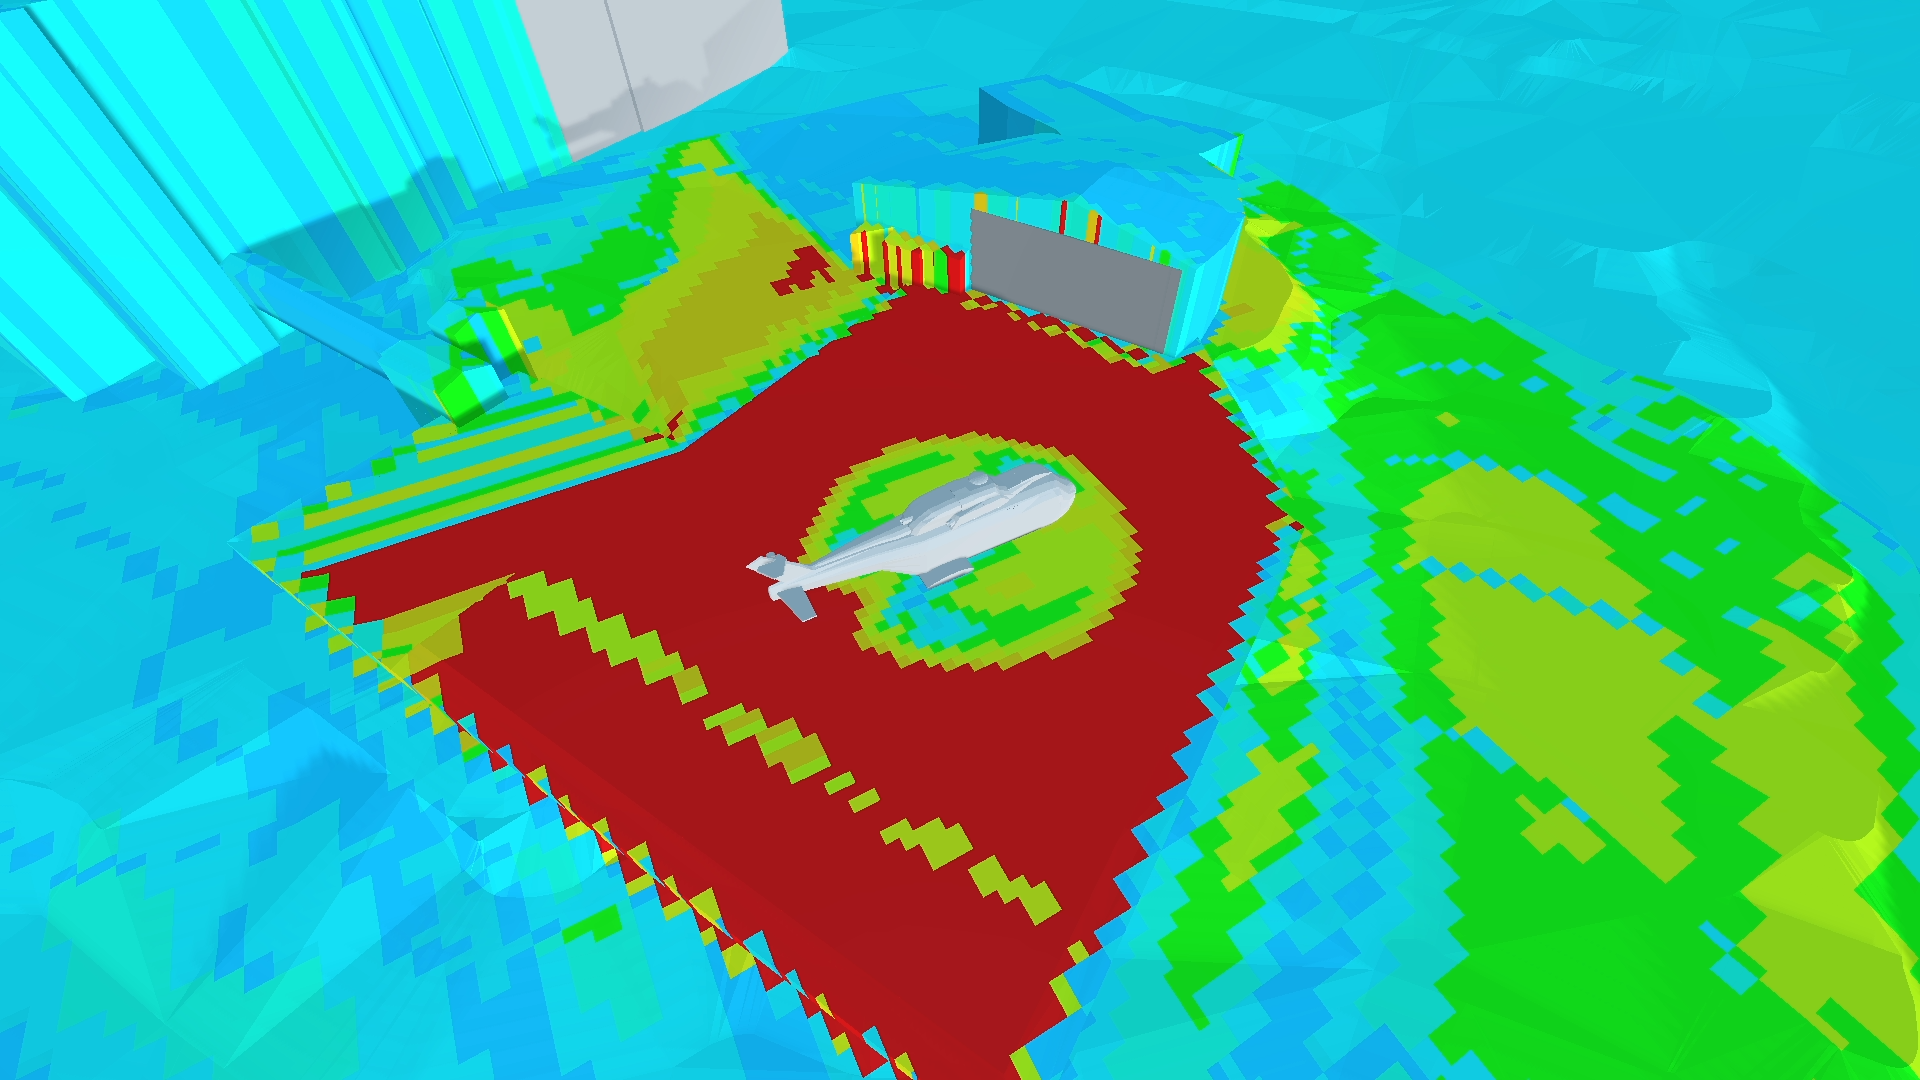
\includegraphics[width=0.8\textwidth]{gfx/anim_heli_last.png}
  \caption{End of Godot animation with the camera attached to the helicopter.}
  \label{fig:AnimHeliLast}
\end{figure}

\begin{figure}[H]
  \centering
  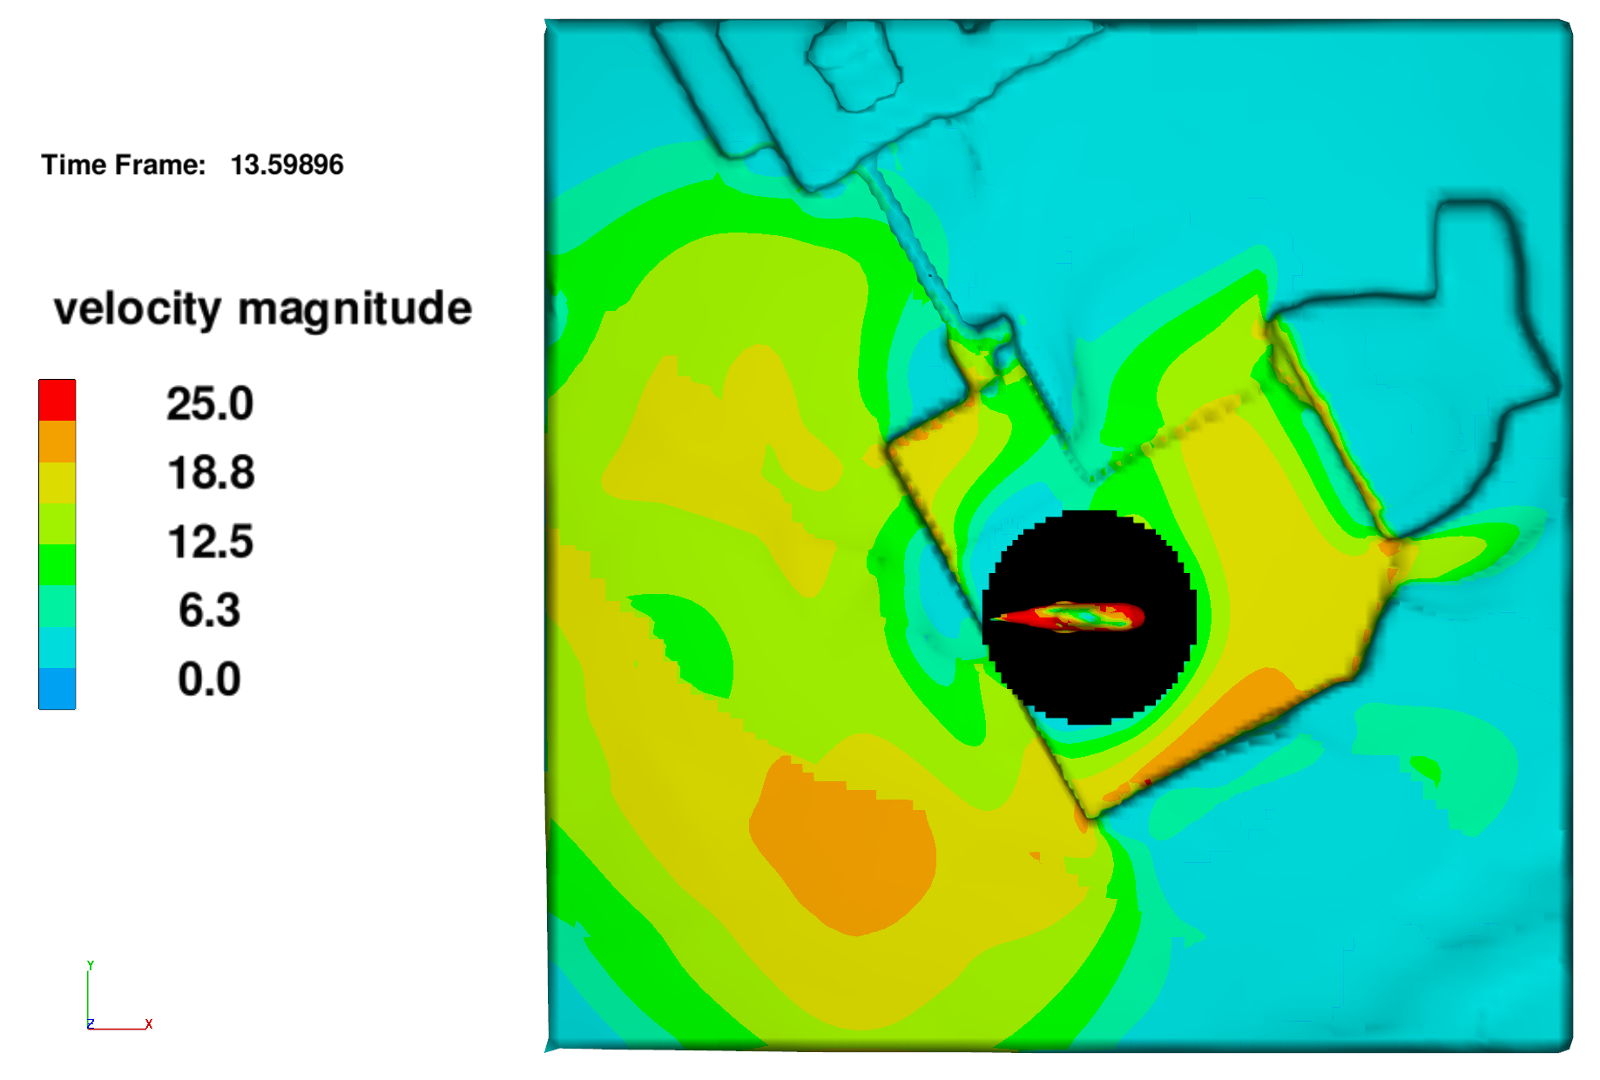
\includegraphics[width=0.8\textwidth]{gfx/flow3d_anim_start.png}
  \caption{Start of FLOW-3D animation.}
  \label{fig:FLOW3DAnimStart}
\end{figure}

\begin{figure}[H]
  \centering
  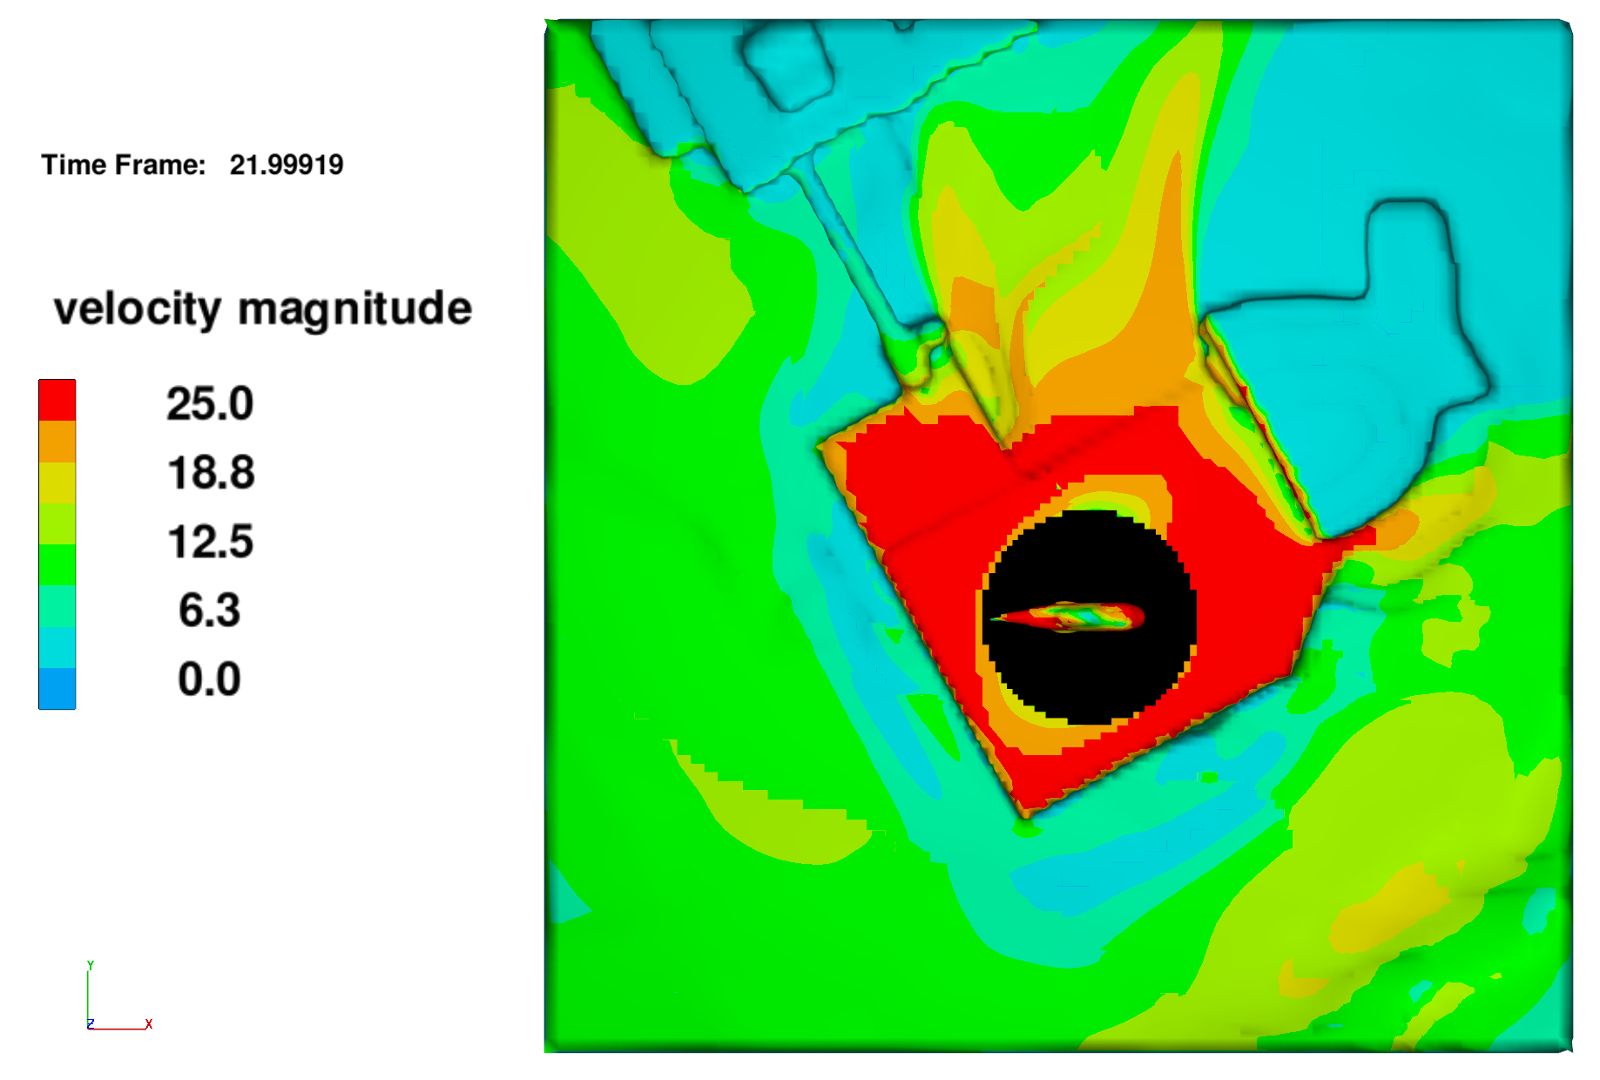
\includegraphics[width=0.8\textwidth]{gfx/flow3d_anim_mid.png}
  \caption{Midpoint of FLOW-3D animation.}
  \label{fig:FLOW3DAnimMid}
\end{figure}

\begin{figure}[H]
  \centering
  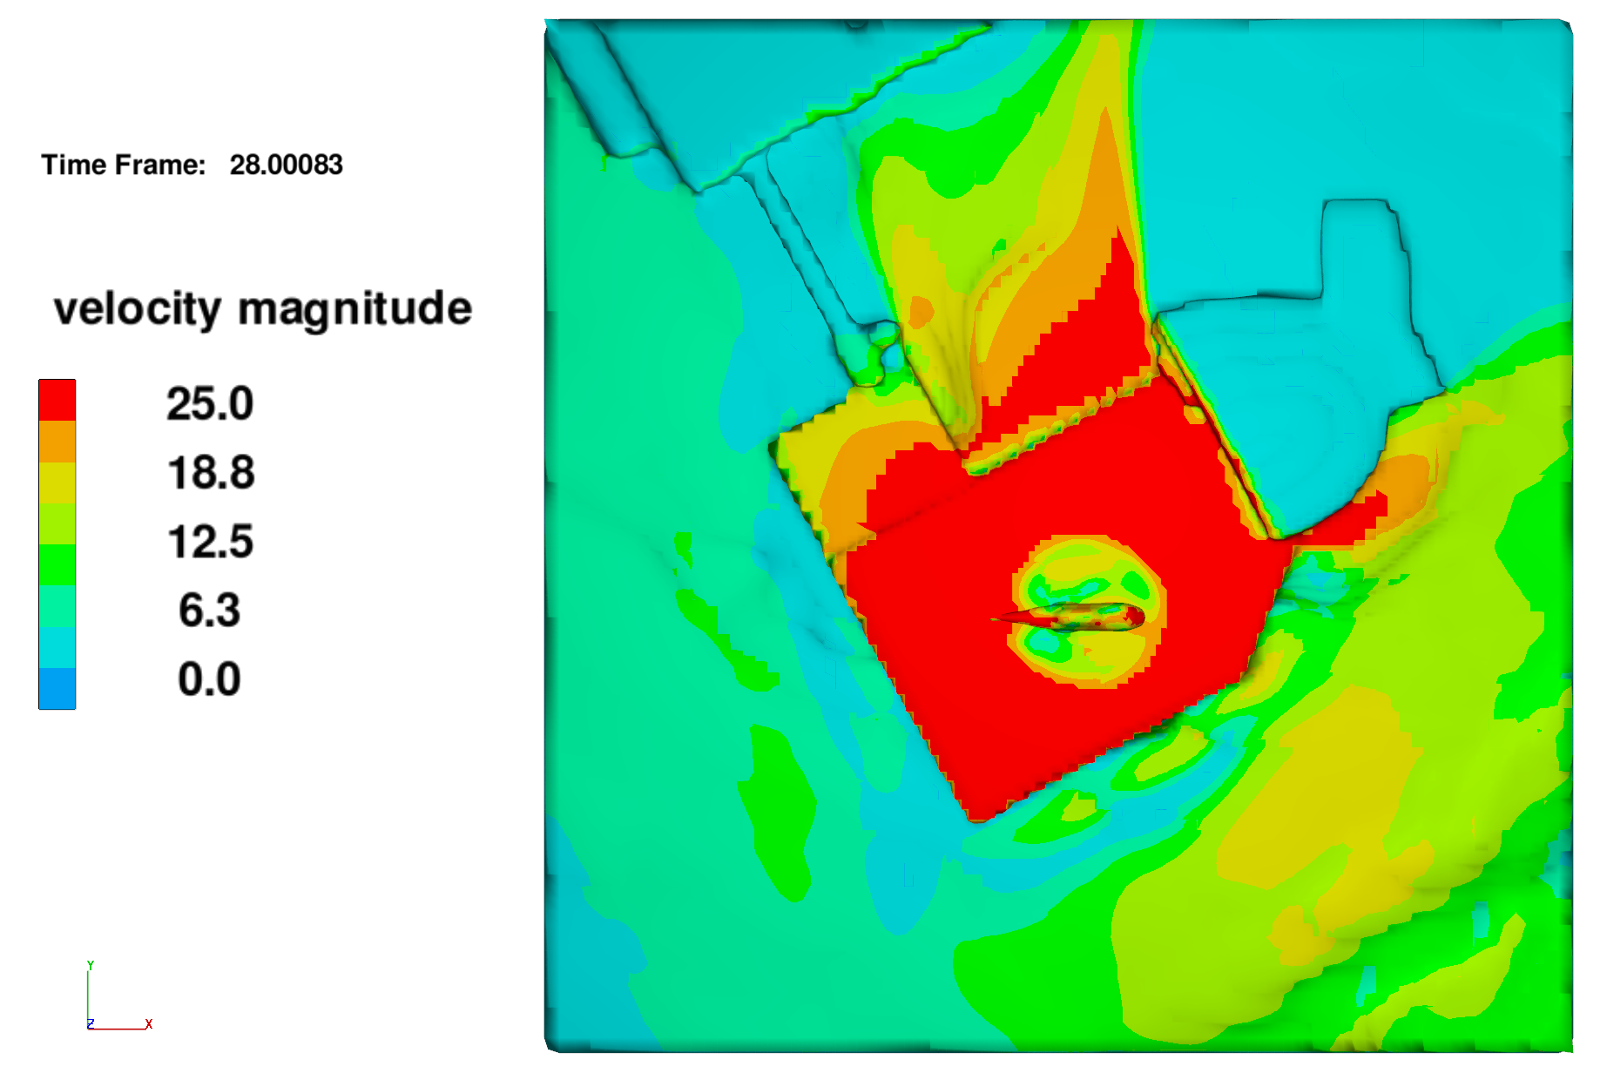
\includegraphics[width=0.8\textwidth]{gfx/flow3d_anim_end.png}
  \caption{End of FLOW-3D animation.}
  \label{fig:FLOW3DAnimEnd}
\end{figure}

Figures \ref{fig:AnimHeliFirst}, \ref{fig:AnimSideMid}, \ref{fig:AnimHeliLast} and the animations in Appendix \ref{app:animations} clearly show how the effect from the helicopter's downdraft on different areas changes over time. We see that the pedestrian areas west and south of the helipad are affected the most during the initial and final stages of the animations. Note that the downdraft's effect on the hangar's gate has not been accounted for in the animation. Furthermore, the entrance to the patient tunnel is affected the most around halfway into the animation. Figures \ref{fig:FLOW3DAnimStart}, \ref{fig:FLOW3DAnimMid} and \ref{fig:FLOW3DAnimEnd} confirm the observations that have been made by providing an alternate form of visualization.
% Something about the gate
% Although the results are clear, there are a few important points to make.

% Small note regarding animation? Linearly interpolated
The helicopter's movement in the Godot animation is linear. This is due to the movement being linearly interpolated between two time steps containing XZ-coordinates. It is possible that partitioning the movement into more steps using data from several time steps, however this was ultimately not pursued due to the amount of time it would take to implement and the minor impact it would have on the results.

% Gaps in textures
In Section \ref{sec:Python} when creating textures, there are gaps in between cells that must be filled. In some cases, such as the top left corner of Figure \ref{fig:PythonTextureGaps}, we see that some gaps can be quite large. The size of such gaps indicates some form of inconsistency in the data that was used, which could be explained by how it was processed with respect to volume fraction. It is possible that edge cases that have not been accounted for exist, e.g. where the volume fraction is 1.0 or 0.0 and the cell is a part of the surface.

The resolution of the textures is quite low. Increasing the resolution would not necessarily have been difficult or very time-consuming, however it would not have made much of an impact on the results, and is more of a cosmetic issue in this case.

% Animations dont add anything new
The animations created in Godot do not necessarily affect any conclusions that can be drawn from the results overall. It would be more accurate to claim that they function as reinforcements. The animation generated in FLOW-3D was completed within minutes, whereas the animations created in Godot were quite complex and time-consuming to complete. This was despite previous experience with both Python and Godot.

% Would have been interesting to use Flowsight for additional post-processing.
Many students from previous years have used FLOW-3D's FlowSight \citep{flowsight} application to perform post-processing. FlowSight is able to produce visualizations with features such as streamlines, which could have been interesting to include in our results. Unfortunately, FlowSight was not installed on the available computer during the project work. Thus, we were unable to produce visualizations with streamlines.

\section{Conclusions}
% Poorly suited for this
Regardless of the points discussed in Section \ref{sec:results}, it is reasonable to suggest the approach taken in this report was successful. Throughout the report, we have visited several interesting concepts such as data processing and texture generation, which have yielded great results.

As illustrated by the figures in Section \ref{sec:results} and the animations in Appendix \ref{app:animations}, we can see that the downdraft caused by the helicopter to the pedestrian areas and the patient entrance to the hospital tunnel varies. The pedestrian areas are affected the most during the initial and final time steps, while the patient entrance is affected the most around halfway in to the animation.

% Future work
% Investigate velocity magnitude on the gate
Possible future work includes to investigate the velocity magnitude on the hangar's gate, which is located toward the side of the helipad. This comes as a natural recommendation, due to it being discussed with professor Per-Arne Sundsbø as a potential part of the task at an early stage of the project. This was ultimately not pursued, due to the project's short time frame and the amount of time that went in to create the report's final result.

\section{Acknowledgements}
Special thanks to my brother Kenneth Wilhelmsen for feedback, advice and inspiration on possible ways to approach the task. I would also like to thank professor Per-Arne Sundsbø for providing the FLOW-3D simulation that was used in the analysis.

\section{References}
\begingroup
\def\section*#1{}
\bibliographystyle{apalike}
\bibliography{References}
\endgroup


%%%%%%%%%%%%%%%%%%%%%%%%%%%%%%%%%%%%%%%
%%      Appendix for the report      %%
%%%%%%%%%%%%%%%%%%%%%%%%%%%%%%%%%%%%%%%

% New Page for appendix
\pagebreak
\begin{appendices}

  % Reset counter for figures, equations, and tables.
  \setcounter{figure}{0}
  \setcounter{table}{0}
  \setcounter{equation}{0}

  % Set numbering for figures, equations and tables A.1, A.2, etc.
  \renewcommand\thefigure{\thesection.\arabic{figure}}
  \renewcommand\thetable{\thesection.\arabic{table}}
  \renewcommand\theequation{\thesection.\arabic{equation}}

  \section{External links}
  This appendix contains external links to the simulation data, models, source code and the full animations from which selected frames have been included in the report.

  \subsection{Simulation data}\label{app:simdata}
  The data from the simulation used as a basis for this report can be found here: \url{https://drive.google.com/drive/folders/1WqYDRVTcwMmO_oYsYifn1NDk9adu7utZ?usp=sharing}. Below is a brief description of its contents:
  \begin{itemize}
    \item \textbf{Directory:} \url{/raw/} --- Raw data exported from FLOW-3D containing vectors for wind velocities at given XYZ-coordinates. Each file contains data for multiple time steps.
    \item \textbf{Directory:} \url{/parsed/} --- Parsed data divided into individual files for each time step. Each file contains XY-coordinates and the length of the associated wind velocity vector.
    \item \textbf{File:} \url{movement.txt} --- The movement of the models in the simulation. Note that in this case, all the models except the helicopter are moving. The buildings and the terrain move towards the helicopter to simulate movement.
  \end{itemize}

  \subsection{Python scripts and models}
  The Python scripts used to process data and create textures can be found at: \url{https://github.com/kribw/fluid-mechanics}. The most notable scripts and their usages are as follows:

  \subsubsection{Processing data}\label{script:process}
  \url{animations/parse_files.py} --- Process data from FLOW-3D and write to individual files for each time step.

  \subsubsection{Determining texture dimensions}\label{script:dimensions}
  \url{animations/parse_input.ipynb} --- Jupyter notebook used for several purposes, one of them being determining the dimensions of the texture.

  \subsubsection{Creating textures}\label{script:texture}
  \url{animations/create_texture.py} --- Create textures from processed data.

  \subsubsection{3D models}\label{app:models}
  \url{/models/} --- 3D models used in simulation and Godot animation. Both \textit{stl} and \textit{glTF} formats are included in separate subdirectories.

  \subsection{Godot project}\label{src:godot}
  The repository for the Godot project used to create the animations can be found at: \url{https://github.com/kribw/VR-H2022/tree/main/fluid_simulations}.

  \textbf{NOTE:} The Godot project will not compile without errors with the code available in the repository, due to a missing model which exceeds GitHub's file size limit of 100 MB. This was discovered while pushing the final changes, right before submitting the report. To compile the project, the missing file \url{Environment.glb} must be downloaded from Appendix \ref{app:simdata} and copied to the \url{/models/} directory.

  \subsection{Animations}\label{app:animations}
  There are three different animations:

  \begin{enumerate}
    \item \url{https://youtu.be/IedGXmY8tm0} --- \textbf{Godot animation}: Camera attached to the helicopter itself.
    \item \url{https://youtu.be/Ptdo3120azE} --- \textbf{Godot animation}: Static camera angle from the side, where we can see the helicopter landing.
    \item \url{https://youtu.be/DvduZhGfeHU} --- \textbf{FLOW-3D animation.}
  \end{enumerate}

\end{appendices}

\end{document}